\section{Virtual Adversarial Training}
\begin{frame}{Virtual Adversarial Training}
Let \(x_*\) represent either a labeled (\(x_l\)) or unlabeled (\(x_{ul}\)) data point.
Our objective function is:
\begin{align*}
&\D{q(y | x_*)}{p(y | x_* + r_{qadv}, \theta)}\\
\text{Where: } &r_{qadv} = \argmax_{r; \norm{r} \le \epsilon} \D{q(y | x_*)}{p(y | x_* + r, \theta)}
\end{align*}
\pause
But we have no information about \(q(y | x_{ul})\).\\
\pause
We'll use its current estimate, \(p(y | x_*, \theta)\) instead (hence the term virtual).
\end{frame}

\begin{frame}{Virtual Adversarial Training}
We denote the current parameters as \(\hat{\theta}\). So the \textit{Local Distributional Smoothness} is defined as:
\begin{align*}
\LDS(x_*, \theta) &= \D{p(y | x_*, \hat{\theta})}{p(y | x_* + r_{vadv}, \theta)}\\
r_{vadv} &= \argmax_{r; \norm{r} \le \epsilon} \D{p(y | x_*, \hat{\theta})}{p(y | x_* + r, \theta)}
\end{align*}

\end{frame}


\begin{frame}{}
The regularization term proposed in the paper is simply the average of \(\LDS\) over all data points:
\begin{align*}
\mathcal{R}(\mathcal{D}_l, \mathcal{D}_{ul}, \theta) = \frac{1}{N_l + N_{ul}} \sum_{x_* \in \mathcal{D}_l, \mathcal{D}_{ul}} \LDS(x_*, \theta)
\end{align*}
    
And the full objective becomes:
\begin{align*}
\mathcal{L} = \ell(D_l, \theta) + \alpha \mathcal{R}(D_l, D_{ul}, \theta)
\end{align*}
\end{frame}

\section{Approximating Virtual Adversarial Direction}

\begin{frame}
\frametitle{Approximating \(r_{vadv}\)}
Assume twice differentiability of \(p(y|x_*, \theta)\) (and as a result \(\divergance\)) with respect to \(x_*\) and \(\theta\).
\(\divergance\) archives the minimum value at \(r = 0\):
\begin{align*}
\divergance(r, x, \hat{\theta})|_{r=0} = 0 \implies \nabla_r \divergance(r, x, \hat{\theta})|_{r=0} = 0
\end{align*}
\pause
The evaluation of \(r_{vadv}\) cannot be performed with the linear approximation as in the original adversarial training since the gradient of \(\divergance(r, x_*, \hat{\theta}) \triangleq\D{p(y | x_*, \hat{\theta})}{p(y | x_* + r, \theta)}\) with respect to \(r\) is always zero at \(r = 0\).
\end{frame}

\begin{frame}
\frametitle{Approximating \(r_{vadv}\)}
We can derive second order Taylor expansion of \(\divergance\) as follows:
\begin{align*}
\divergance(r, x, \hat{\theta}) \approx \frac{1}{2} r^T H(x, \hat{\theta})r
\end{align*}

Where \(H(x, \hat{\theta})\) is the Hessian matrix of \(\divergance\) with respect to \(r\).\\

\pause

We know that the maximum value of \(\divergance\) is achieved when \(r\) is the eigenvector \(u(x, \hat{\theta})\) of the matrix \(H\) corresponding to the largest eigenvalue:
\begin{align*}
r_{vadv} &\approx \argmax_r\left\{r^T H(x, \hat{\theta})r \mid \norm{r} \le \epsilon\right\}\\
&= \epsilon \overline{u(x, \hat{\theta})} \tag{\(\overline{v} = \frac{v}{\norm{v}}\)}
\end{align*}
\end{frame}

\begin{frame}
    \frametitle{Approximating \(r_{vadv}\)}
What about \(O(I^3)\) complexity of computing the eigenvector?

\pause
We use the iterative \textit{Power Method} to approximate the dominant eigenvector.
Suppose \(d\) is a random unit vector. If \(d\) is not prependicular to the dominant eigenvector, then iterative calculation of
\begin{align*}
d \leftarrow \overline{Hd}
\end{align*}
converges to the dominant eigenvector (see~\nameref{sec:appendix}).
\end{frame}

\begin{frame}
\frametitle{Approximating \(r_{vadv}\)}
We can approximate \(Hd\) with difference method too:
\begin{align*}
Hd &\approx \frac{\nabla_r \divergance(r, x_*, \hat{\theta})|_{r=\xi d} - \nabla_r \divergance(r, x_*, \hat{\theta})|_{r=0}}{\xi}\\
&= \frac{\nabla_r \divergance(r, x_*, \hat{\theta})|_{r=\xi d}}{\xi}
\end{align*}
\pause 
\begin{align*}
\implies d \leftarrow \overline{\nabla_r \divergance(r, x_*, \hat{\theta})|_{r=\xi d}}&&
\end{align*}
Thus, the approximation of \(r_{vadv}\) with \(K\) steps of the power method can be achieved with \(K\) sets of backpropagation.
\end{frame}

\begin{frame}
\frametitle{Approximation for Derivative of Regularization Term}
\begin{center}
\begin{minipage}{0.9\linewidth}
\begin{algorithm}[H]
\caption{Mini-batch SGD for \(\nabla_\theta\mathcal{R}\) with one time iteration of power method}
Choose \(M\) random samples from dataset \(\mathcal{D}\): \(\left\{x^{(i)}\right\}_{i=1}^M\).\\
Sample unit vector \(d^{(i)}\) from an iid Gaussian distribution.\\
Calculate \(r_{vadv}\) with one set of backpropagation:
\begin{align*}
g^{(i)} &\gets \left.\nabla_r \D{p(y | x^{(i)}, \hat{\theta})}{p(y | x^{(i)} + r, \theta)}\right|_{r=\xi d^{(i)}}\\
r_{vadv}^{(i)} &\gets \epsilon \frac{g^{(i)}}{\norm{g^{(i)}}}
\end{align*}\\
\Return{\(\nabla_\theta \left(\frac{1}{M}\sum_{i=1}^M \D{p(y | x^{(i)}, \hat{\theta})}{p(y | x^{(i)} + r_{adv}^{(i)}, \theta)}\right)\)}
\end{algorithm}
\end{minipage}
\end{center}
\end{frame}

\subsection{Tuning Hyperparameters}
\begin{frame}
    \frametitle{Tuning Hyperparameters}

We have two hyperparameters: \(\epsilon\) and \(\alpha\).

\begin{align*}
\max_r\left\{ \divergance(r, x, \theta) \mid \norm{r}_2 \le \epsilon\right\} & \approx \max_r\left\{\frac{1}{2} r^T H(x, \theta)r \mid \norm{r}_2 \le \epsilon\right\}\\
& = \frac{1}{2} \epsilon^2 \lambda_1(x, \theta)
\end{align*}
    
\pause
\begin{align*}
\mathcal{L} &= \ell(\theta, \mathcal{D}_l) + \alpha \mathcal{R}_{vadv} (\theta, \mathcal{D}_l, \mathcal{D}_{ul})\\
&= \ell(\theta, \mathcal{D}_l) + \alpha \frac{1}{N_l + N_{ul}} \sum_{x \in \mathcal{D}_l, \mathcal{D}_{ul}} \max_r\left\{ \divergance(r, x, \theta) \mid \norm{r}_2 \le \epsilon\right\}\\
& \approx \ell(\theta, \mathcal{D}_l) + \frac{1}{2} \epsilon^2\alpha \frac{1}{N_l + N_{ul}} \sum_{x \in \mathcal{D}_l, \mathcal{D}_{ul}}  \lambda_1(x, \theta)
\end{align*}

\end{frame}

\section{Experiments}

\begin{frame}
    \frametitle{Experiments}
\begin{align*}
\divergance =& \text{KL Divergence}\\
\xi =& 10^{-6}\\
\alpha =& 1\\
\text{Model} =& \text{Simple Fully Connected Network with 4 hidden layers}\\&\text{ for MNIST and Conv-Large for CIFAR-10}
\end{align*}
\end{frame}

\begin{frame}
    \frametitle{Experiments}
\begin{table}
\centering
\caption{Test performance of supervised learning methods
on MNIST with 60,000 labeled examples in the permutation
invariant setting.}
\label{tab:mnist}
\begin{tabular}{l r}
\hline
\hline
Method & Test error rate(\%)\\
\hline
SVM (Gaussian kernel) & 1.40\\
Dropout  & 1.05\\
Adversarial, \(L_\infty\) norm constraint &  0.78\\
Ladder networks &  0.57 (\(\pm\)0.02)\\
\hline
Baseline (MLE) & 1.11 (\(\pm\)0.06)\\
RPT & 0.84 (\(\pm\)0.03)\\
Adversarial, \(L_1\) norm constraint &0.79 (\(\pm\)0.03)\\
Adversarial, \(L_2\) norm constraint& 0.71 (\(\pm\)0.03)\\
VAT &0.64 (\(\pm\)0.05)\\
\hline
\hline
\end{tabular}
\end{table}
\end{frame}

\begin{frame}
    \frametitle{Experiments}

\begin{table}
\centering
\caption{Test performance of supervised learning methods
implemented with CNN on CIFAR-10 with 50,000 labeled
examples.}
\label{tab:ciphar10}
\begin{tabular}{l r}
\hline
\hline
Network in Network & 8.81\\
All-CNN & 7.25\\
Deeply Supervised Net & 7.97\\
Highway Network & 7.72\\
ResNet (1001 layers) & 4.62 (\(\pm\)0.20)\\
DenseNet (190 layers) & 3.46\\
\hline
Baseline (only with dropout) &6.67 (\(\pm\)0.07)\\
RPT &6.30 (\(\pm\)0.04)\\
VAT &5.81 (\(\pm\)0.02)\\
\hline
\hline
\end{tabular}
\end{table}

\end{frame}


\begin{frame}
\frametitle{Experiments}
\vspace{-1em}
\begin{table}
\centering
\caption{Test performance of semi-supervised learning
methods.}
\label{tab:semi}
\resizebox{0.75\columnwidth}{!}{%
\begin{tabular}{l r r}
\hline
\hline
\multirow{3}{*}{Method} & \multicolumn{2}{c}{Test error rate(\%)}\\
& SVHN & CIFAR-10 \\
& \(N_l = 1000\) & \( N_l = 4000\)\\
\hline
SWWAE & 23.56&\\
% *Auxiliary DGM & 22.86&\\
% *Skip DGM & 16.61 (\(\pm\)0.24)&\\
Auxiliary DGM & 22.86&\\
Skip DGM & 16.61 (\(\pm\)0.24)&\\
Ladder networks, \(\Pi\) model && 20.40 (\(\pm\)0.47)\\
CatGAN && 19.58 (\(\pm\)0.58)\\
GQAN with FM & 8.11 (\(\pm\)1.3) &18.63 (\(\pm\)2.32)\\
model & 5.43 (\(\pm\)0.25) &16.55 (\(\pm\)0.29)\\
\hline
(on Conv-Small) & & \\
RPT & 8.41 (\(\pm\)0.24) & 18.56 (\(\pm\)0.29)\\
VAT & 6.83 (\(\pm\)0.24) & 14.87 (\(\pm\)0.13)\\
\hline
(on Conv-Large) & & \\
VAT & 5.77 (\(\pm\)0.32) & 14.18 (\(\pm\)0.38)\\
VAT+EntMin & 4.28 (\(\pm\)0.10)  & 13.15 (\(\pm\)0.21)\\
\hline
\hline
\end{tabular}%
}
\end{table}
\end{frame}

\begin{frame}
    \frametitle{Conditional Entropy Minimization}
VAT + \underline{EntMin}:
\begin{align*}
\mathcal{R}_{cent} &= \mathcal{H}(Y|X)\\
&= -\frac{1}{N_l + N_{ul}} \sum_{x\in \mathcal{D}_l, \mathcal{D}_{ul}}\sum_{y} p(y|x, \theta) \log p(y|x, \theta)
\end{align*}
\end{frame}

\begin{frame}
\frametitle{Performance of VAT with different \(\epsilon\)}
\begin{figure}
\centering
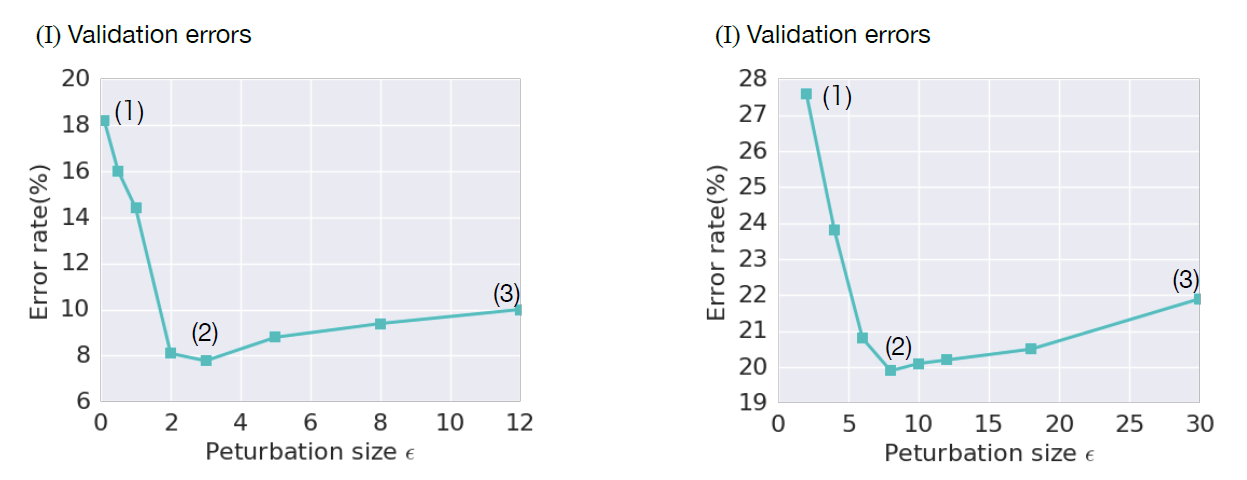
\includegraphics[width=0.8\columnwidth]{different_eps_val.png}
\caption{Validation error rate of VAT with different \(\epsilon\) on SVHN and CIFAR-10.}
\label{fig:different_eps_val}
\end{figure}
\end{frame}

\begin{frame}
\frametitle{Performance of VAT with different \(\epsilon\)}
\begin{figure}
\centering
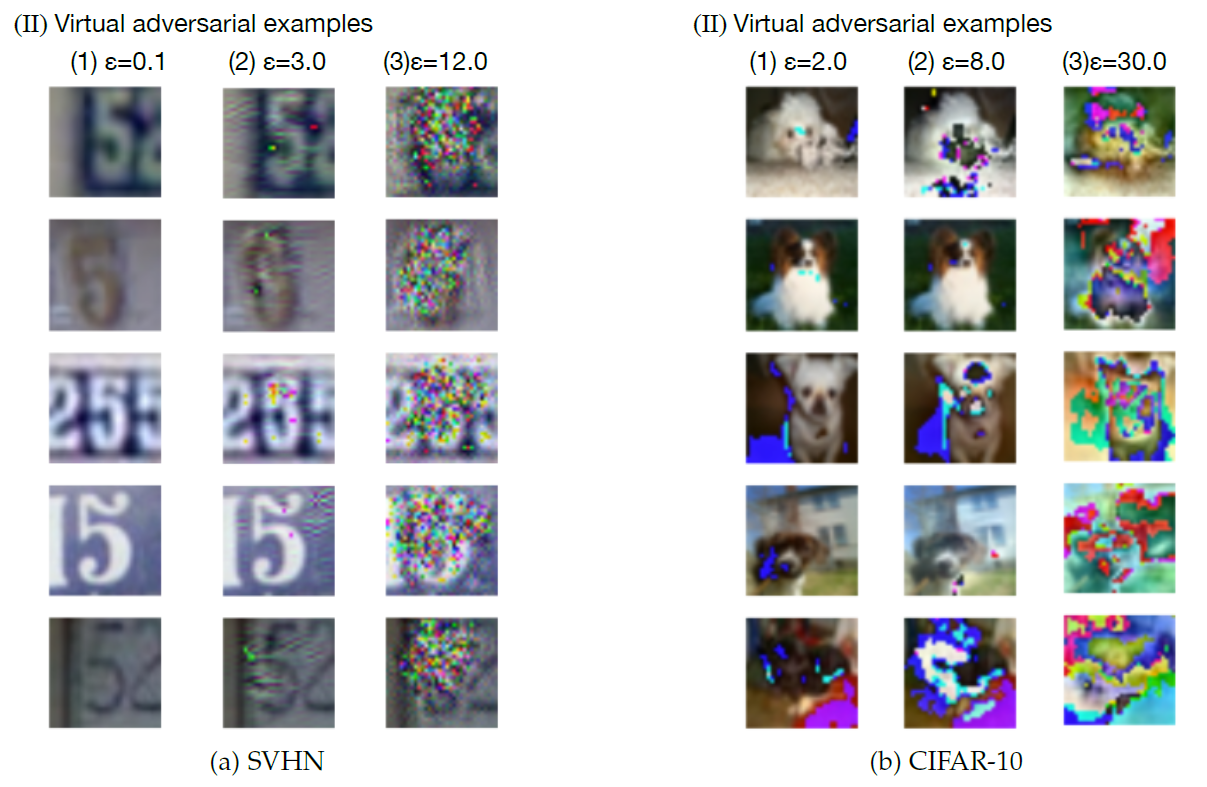
\includegraphics[width=0.8\columnwidth]{different_eps_images.png}
\caption{Images distorted with \(r_{vadv}\) with different \(\epsilon\) on SVHN and CIFAR-10.}
\label{fig:different_eps_images}
\end{figure}
\end{frame}

\begin{frame}
\frametitle{Conclusion}
\begin{itemize}
\item Effective model for both supervised and semi-supervised learning on different datasets
\item Small computational cost
\item Model agnostic
\item Simple:
\begin{itemize}
\item Requires optimization of only one hyperparameter
\item Does not require training of additional models
\end{itemize}
\end{itemize}

\end{frame}